\part{Interference}
    \section{Superposition Again}
    Consider two beams of light from two point sources, \(S_1\) and \(S_2\), which are separated by some distance \(a\), propagating in an \gls{lih} medium.
    We assume that the two sources have the same angular frequency, \(\omega\), and that \(a \gg \lambda\).
    At some point \(P\), far from the two sources we effectively have plane waves:
    \[\vv{E_i} = \vv{E_{0i}}\cos(\vv{k_i\cdot\vv{r} - \omega t - \Phi_i}).\]
    The net field at this point is
    \[\vv{E} = \vv{E_1} + \vv{E_2}.\]
    As usual \(E\) oscillates far too quickly to be a useful quantity to measure.
    Instead we are interested in the intensity,
    \[I = \varepsilon v\expected{E^2}.\]
    Here \(\varepsilon = \varepsilon_0\varepsilon_r\) and \(v\) is the speed of light in this medium.
    If the intensity of each source at this point is \(I_i\) then we find that the intensity of the combined light is
    \begin{align*}
        I &= \varepsilon v\expected{E_1^2 + E_2^2 + 2\vv{E_1}\cdot\vv{E_2}}\\
        &= I_1 + I_2 + 2\varepsilon v\expected{\vv{E_1}\cdot\vv{E_2}}\\
        &= I_1 + I_2 + 2\varepsilon v\vv{E_{01}}\cdot\vv{E_{02}}\expected{\cos(\vv{k_1}\cdot\vv{r} - \omega t - \Phi_1)\cos(\vv{k_2}\cdot\vv{r} - \omega t - \Phi_2)}.
    \end{align*}
    So the resulting intensity is the sum of the two intensities plus an interference term, \(I_{12}\).
    We can evaluate this term by noticing that \(\expected{\sin^2\vartheta} = \expected{\cos^2\vartheta} = 1/2\) and \(\expected{\sin\vartheta\cos\vartheta} = 0\) so
    \[I_{12} = 2\varepsilon v\vv{E_{01}}\cdot\vv{E_{02}}\cos \delta\]
    where
    \[\delta = (\vv{k_1} - \vv{k_2})\cdot\vv{r} - \Phi_1 + \Phi_2.\]
    It follows from this that if \(\vv{E_{01}}\) and \(\vv{E_{02}}\) are orthogonal then the interference term vanishes and \(I = I_1 + I_2\) whereas if \(\vv{E_{01}}\) and \(\vv{E_{02}}\) are parallel then we have
    \[I = I_1 + I_2 + 2\sqrt{I_1I_2}\cos\delta.\]
    Then for the specific case of \(\delta = 2n\pi\) for \(n\in\integers\) we have \define{total constructive interference} and \(I\) is maximised:
    \[I = I_1 + I_2 + 2\sqrt{I_1I_2}.\]
    On the other hand if \(\delta = (2n + 1)\pi\) then we have \define{totally destructive interference} and the intensity is minimised:
    \[I = I_1 + I_2 - 2\sqrt{I_1I_2}.\]
    Often we will see patterns where we have both constructive and destructive interference, called \define{fringes}.
    A useful quantity to define is the \define{fringe contrast}:
    \[C = \frac{\max\{I\} - \min\{I\}}{\max\{I\} + \min\{I\}}.\]
    This is easily measured.
    It can be shown that \(C\) is maximised by the case of \(I_1 = I_2\).
    
    It is only possible to view fringes if \(\delta\) is stable.
    In practice this means that the phase difference, \(\Phi_1 - \Phi_2\) has to be stable.
    This is not the case for everyday light sources which is why we need to set up special lab conditions with lasers and slits in order to start seeing fringes.
    
    At the start of this section we specified that \(a \gg \lambda\).
    This is required for the two sources to act as two separate sources.
    The result is that \(I_{12}\) averages to zero over all space and so the effect of interference is to increase the energy at some points and decrease it at others.
    If \(a \sim \lambda\) then the two sources behave more like one source with amplitude \(E_{01} + E_{02}\).
    
    \section{Films}
    When testing Fresnel's equations physicist Lord Rayleigh found that they only held for freshly prepared glass.
    The conclusion was that some oxidation process lead to a film on the glass which changed the optical properties.
    Counter to what one may expect this layer of tarnish actually increased the transmission of the glass.
    
    If light travels from medium 1 to medium 3 at normal incidence then we have seen that the reflection coefficient is
    \[R_{13} = \abs{\frac{n_1 - n_3}{n_1 + n_3}}^2.\]
    We will now consider what happens if we include a thin layer of medium 2 in between media 1 and 3.
    For simplicity we will take medium 1 to be air and medium 3 to be glass.
    We will also assume that the transmission coefficient of the film is high and the reflection coefficient is low.
    For enhanced transmission it we must have decreased reflection.
    In fact it is the reflection that is decreased by this scenario and the increased transmission is simply a side effect.
    
    The mechanism by which this occurs is as follows:
    \begin{itemize}
        \item The beam of light enters the film.
        A small portion is reflected with intensity \(I_0R_{12}\) but most passes through. The intensity of the transmitted beam is \(I_0T_{12}\).
        \item The beam reaches the glass and a small portion is reflected again.
        The intensity of this reflection is \(I_{0}T_{12}R_{13}\).
        \item This beam reaches the film-air boundary and is transmitted with intensity \(I_{0}T_{12}^2R_{13}\) (note that \(T_{12} = T_{21}\)).
    \end{itemize}
    In theory part of this beam reflects back to the glass, then is reflected back to the film-air boundary and part of this is transmitted and so on but for very clear materials the reflectivity is low enough that we can neglect secondary reflections.
    Yet another approximation we can make is \(T_{12} \approx 1\) and so the net intensity of the reflected light is \(I_0(R_{12} + R_{23})\).
    For the case of \(n_1 < n_2 < n_3\) the net reflectivity, \(R_{12} + R_{23}\), is lower than the reflectivity of the air-glass boundary.
    Notice that \(R\) scales quadratically with \(\Delta n\) so if the film has a refractive index somewhere between the two other mediums then \(\Delta n\) is decreased at each step and since it is squared this has the effect of reducing the overall reflectivity since if \((\Delta n_{13})^2 = (\Delta n_{12} + \Delta n_{23})^2 = \Delta n_{12}^2 + \Delta n_{23}^2 + 2\Delta n_{12}\Delta n_{23} < \Delta n_{12}^2 + \Delta n_{23}^2\) since all \(\Delta n\) have the same sign if \(n_1 < n_2 < n_3\).
    
    We can take this to the extreme and use many thin layers all only with slightly higher refractive index than the last and increase transmissivity by a lot.
    The limiting case is then a medium with smoothly changing refractive index which experiences no reflection.
    This is exploited in optical fibres to bend light away from the outside rather than having an abrupt reflection.
    This helps signals stay together as they follow more similar paths.
    
    \subsection{Thin Film Interference}
    In the previous section we assumed that the two reflected beams didn't interfere.
    This is a reasonable assumption if the thickness of the film is greater than the coherence length of the light.
    If this isn't the case then the thickness of the film determines the number of wavelengths that the two beams travel before coming together and this in turn determines whether there will be constructive or destructive interference.
    
    Of particular interest is when we can use destructive interest to reduce the reflectivity (and hence increase transmissivity) of a material.
    If the film has physical thickness \(d\) the for light of wavelength \(\lambda\) we define the phase thickness to be \(\beta = 2\pi n_2d/\lambda\).
    The reflection coefficient for the system is
    \[r_{123} \approx r_{12} + e^{i\beta}r_{23}e^{i\beta}.\]
    Here \(r_{12}\) gives the initial reflection off of the air-film boundary and \(r_{23}\) gives the reflection off of the film-glass boundary.
    There are then two factors of \(e^{i\beta}\) as the reflected wave must travel through the film twice (once in each direction).
    The reason this is only approximate is we are ignoring secondary reflections.
    To minimise reflection we use a film with refractive index, \(n_2\), somewhere between that of air and glass.
    The question of interest is what physical thickness of film do we need?
    To answer this question it is important to note that both reflections occur when in a low refractive index material and reflecting off of a higher refractive index material.
    This means that both reflections cause a phase shift of \(\pi\), the actual value of this phase shift is not important, what is important is it is the same for both so actually has no effect on the type of interference.
    If instead we had \(n_2\) be higher then the refractive index of glass then we would need to consider more carefully the phase shift due to reflection.
    
    Noticing that the equation can be written as
    \[r_{123} \approx r_{12} + e^{2i\beta}r_{23}\]
    we see that choosing \(\beta = \pi/2\) results in destructive interference, so we choose \(d = \lambda/(4n_2)\).
    We now just have to choose a value for \(n_2\) which we can do by expanding the Fresnel coefficients:
    \[r_{123} \approx r_{12} - r_{23} = \frac{n_1 - n_2}{n_1 + n_2} - \frac{n_2 - n_3}{n_2 + n_3}\]
    which will be zero if \(n_2 = \sqrt{n_1n_3}.\)
    So for an air-glass system taking \(n = 1\) for air and \(n = 1.5\) for glass we have \(n_2 = 1.22\).
    In reality there is not a material with the required refractive index and other physical attributes needed to form a thin film.
    It is common to use \ce{MgF_2} which has \(n = 1.38\).
    The reflectivity can then be reduced from \(\SI{4}{\percent}\) to \(\SI{1.5}{\percent}\).
    It is possible to do better if we use multiple layers of thin films and exploit the phase difference that is accrued when reflecting off of a high refractive index material but not a low refractive index material.
    
    \subsection{Soap Film}
    Consider a soap film stretched over a wire frame as shown in figure~\ref{fig:soap film}.
    If this frame is vertical then gravity will stretch the soap downwards causing the film to be thicker at the bottom and thinner at the top.
    In a similar way to the last section we can consider only the first order reflections off of the soap-air and air-soap boundaries.
    The refractive index of the soap film will be greater than that of air and so the air-soap reflection will have a phase shift of \(\pi\) and the soap-air reflection will not.
    At the top of the film, the thinnest part if the thickness \(d_1 < \lambda\) then the phase thickness is \(\delta \approx \pi\) due to the phase shift upon reflection.
    This results in destructive interference and the top of the film appears black.
    Further down when the thickness is \(d_2 > \lambda\) the phase thickness will be
    \[\delta = \frac{4d_2n}{\lambda_0} + \pi.\]
    Here \(\lambda_0\) is the wavelength of light we are interested in.
    We have constructive interference at this wavelength when \(\delta = 2\pi m\) for \(m\in\integers\).
    As we move down the film and the thickness increases all colours in the spectrum will eventually interfere constructively at some point and so we see the entire spectrum.
    We then see the entire spectrum again for the next value of \(m\) and so on until the thickness of the soap film is greater than the coherence length at which point we just see white.
    \begin{figure}[htbp!]
        \centering
        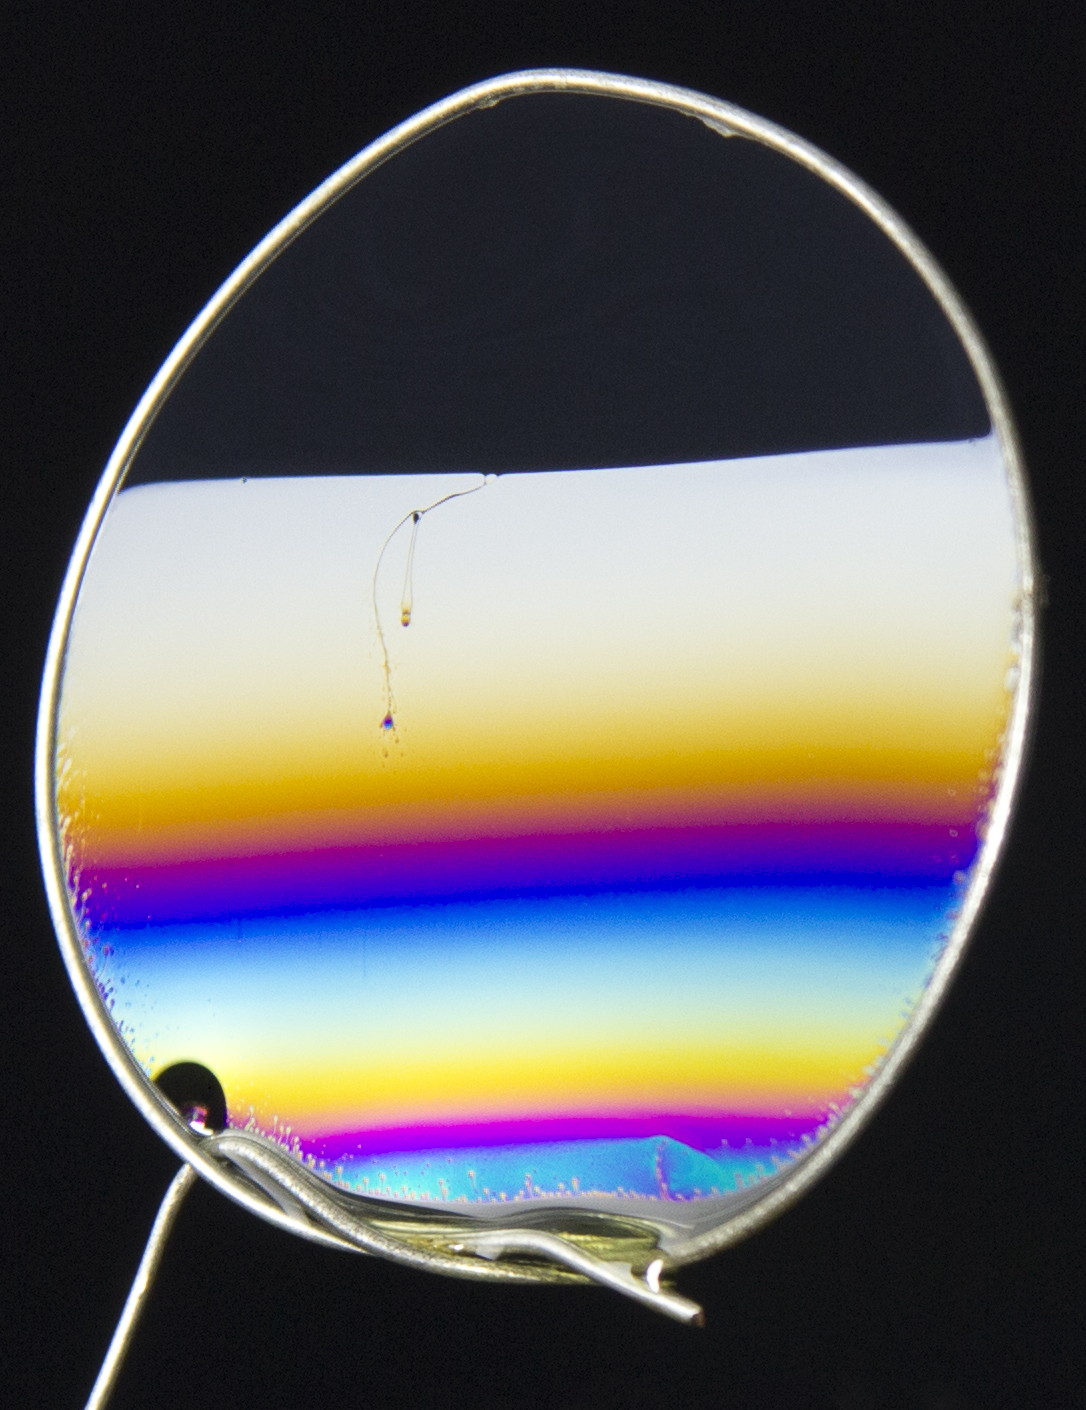
\includegraphics[scale=1]{soapfilm.jpg}
        \caption{A soap film showing destructive interference at the top due to a phase shift upon reflection and a spectrum lower down due to varying thickness. Image credit: \url{https://www.animations.physics.unsw.edu.au/jw/light/soap-bubbles.htm} accessed on 27/04/2021.}
        \label{fig:soap film}
    \end{figure}
    
    \subsection{Newton's Rings/Newton's Wedge}
    Newton's rings and Newton's wedge are related phenomena where a slowly increasing gap between two glass components causes a pattern of fringes, see figure~\ref{fig:newtons wedge and rings}.
    Newton's wedge uses two flat pieces of glass laid on top of each other with the upper piece being raised slightly on one side such that the gap between the two pieces is wedged shaped see figure~\ref{fig:newtons wedge}.
    Newton's rings uses a planar-convex of radius \(R\) with the lens placed convex side down on a flat glass surface so that moving away from the centre results in the space between the lens and the glass increases as you move away fro m the centre of the lens, see figure~\ref{fig:newtons rings}.
    The result of both of these is that incident light is split, ignoring second order reflections and reflections off of a glass-air boundary there will be two beams that leave the setup.
    
    For Newton's wedge the way that this works is the first beam reflects off of the first air-glass boundary and the second makes it through this boundary and into the small space between the two pieces of glass before reflecting off of the next air-glass boundary.
    Consider Newton's wedge and in particular pick two adjacent bright fringes along the wedge such that the size of the air gap is \(d_a\) at the first point and \(d_b\) at the second.
    The phase thickness is then \(\beta_a = 2\pi d_a/\lambda\) at the first point and \(\beta_b = 2\pi d_b/\lambda\) at the second.
    If the distance between the two points is \(\Delta x\) then simple geometry gives us
    \[\tan\alpha = \frac{d_b - d_a}{\Delta x} = \frac{\lambda}{2\Delta x} \implies \Delta x = \frac{\lambda}{2\tan\alpha} \approx \frac{\lambda}{2\alpha}.\]
    
    Consider now Newton's rings.
    In this case we have normal incidence on the top plane of the lens.
    The two beams that interact this time are the beam that reflects off of the convex face of the lens and the beam that reflects off the glass block below.
    At a distance \(r\) from the centre of the lens the thickness of the air gap is \(d\).
    Taking the convex side of the lens to be part of a sphere we have that
    \[(R - d)^2 + r^2 = R^2 \implies r^2 = 2Rd - d^2 \implies d \approx \frac{r^2}{2R}\]
    where the approximation assumes that \(d \ll R\).
    This equates to approximating the spherical lens face as parabolic.
    The phase shift between the two beams is twice the thickness of this air gap minus \(\pi\) due to the phase change upon reflection at the glass-air boundary.
    \[\delta = 2 \cdot 2\pi\frac{d}{\lambda} - \pi = \frac{2\pi r^2}{R\lambda} - \pi.\]
    We get bright fringes when \(\delta = 2m\pi\) for \(\pi\in\integers\) so bright fringes occur at distances
    \[r_m = \sqrt{\left( m + \frac{1}{2} \right)\lambda R}.\]
    Notice that at the centre, \(r = 0\), we get a dark fringe due to the fact that there is no boundary at the centre where the two glass components touch and therefore no reflection.
    \begin{figure}[htbp!]
        \centering
        \begin{subfigure}[b]{0.45\textwidth}
            \centering\tikzexternaldisable
            \tikzsetnextfilename{Newtons-wedge}
            \begin{tikzpicture}
                \tikzset{glass/.style={blue!25}}
                \tikzset{light/.style={red, thick}}
                \fill[glass] (0, 0) rectangle (4, -0.2);
                \fill[glass, rotate=10] (0, 0) rectangle (4, 0.2);
                \begin{scope}
                    \clip (0, 0) rectangle (1.5, 0.95);
                    \draw[light] (0.7, 1) -- (1, 0) -- (1.3, 1);
                    \draw[light, xshift=-0.05cm, yshift=0.17cm] (1, 0) -- (1.3, 1);
                \end{scope}
            \end{tikzpicture}
            \caption{Newton's Wedge}
            \label{fig:newtons wedge}
        \end{subfigure}
        \begin{subfigure}[b]{0.45\textwidth}
            \centering
            \tikzsetnextfilename{Newtons-rings}
            \begin{tikzpicture}
                \tikzset{glass/.style={blue!25}}
                \tikzset{light/.style={red, thick}}
                \fill[glass] (0, 0) rectangle (4, -1);
                \begin{scope}
                    \clip (0, 0) rectangle (4, 0.8);
                    \fill[glass] (2, 4) circle[radius=4];
                \end{scope}
                \draw[light] (1, 1.75) -- (1, 0);
                \draw[light, ->, >=latex] (1, 0.5) -- (1, 0.49);
                \begin{scope}
                    \clip (2, 4) circle[radius=4];
                    \draw[light, ->, >=latex] (1.1, 0) -- (1.1, 1.5);
                \end{scope}
                \draw[light, ->, >=latex] (0.9, 0) -- (0.9, 1.5);
                \draw[|-|] (1, -0.3) -- (2, -0.3) node[midway, below] {\(r\)};
                \draw[|-|] (2, 0) -- (2, 4) node[midway, right] {\(R\)};
                \draw[->, >=latex] (2, 4) -- (1, 0.125) node[midway, left] {\(R\)};
                \draw[dashed] (1, 0.125) -- (0, 0.125);
                \draw[|-|] (0, 0.13) -- (0, 0) node[midway, left] {\(d\)};
            \end{tikzpicture}
            \caption{Newton's Rings}
            \label{fig:newtons rings}
        \end{subfigure}
        \caption{Newton's Wedge and Newton's Rings create a series of bright and dark fringes through a similar mechanism of a gradually increasing air gap.}
        \label{fig:newtons wedge and rings}
    \end{figure}
    
    \subsection{Films to Increase/Decrease Reflectivity}
    By cleverly layering films it is possible to dramatically change the reflectivity of a material.
    The simplest example involves two layers of film onto glass, first a low refractive index layer and then a high refractive index layer.
    This way light has to pass from air to low, to high, to glass.
    Each time the light passes through one of these boundaries the refractive index is relatively higher and therefore the light that is reflected picks up a phase shift of \(\pi\).
    By constructing these layers to be the correct thickness it is possible to have destructive interference for the light that is reflected off of the different layers decreasing reflectivity and increasing transmissivity.
    
    Similarly a system of alternating low and high refractive index films can encourage many reflections which, if the thickness of the layers is correct, interfere constructively resulting in high reflectivity which allows us to make a mirror out of a transparent medium.
    
    \section{More Thin Film}
    \subsection{Non-Normal Incidence}
    Consider a bubble.
    When viewed at the right angle the bubble will appear multicoloured.
    This is due to thin film effects.
    The colours also change as the thickness of the bubble is not constant.
    More interestingly the colours also change based on the angle of viewing which is an effect known as \define{iridescence} which we will study in this section.
    
    \begin{figure}[ht]
        \centering
        \begin{tikzpicture}
            \tikzset{film/.style={blue!25}}
            \tikzset{light/.style={red, very thick}}
            \fill[film] (0, 0) rectangle (1, 4);
            \begin{scope}
                \clip (1, 2) -- (4, 4) -- (2, 2) -- cycle;
                \draw (1, 2) circle[radius=0.5];
            \end{scope}
            \node at (1.7, 2.2) {\(\vartheta_i\)};
            \draw[light] (4, 4) -- (1, 2);
            \draw[light, ->, >=latex] (1, 2) -- (4, 0);
            \draw[light, ->, >=latex] (0, 1.75) -- (1, 1.5) -- (4, -0.5);
            \draw[light, ->, >=latex] (1, 2) -- (0, 1.75) -- (-2, 0);
            \begin{scope}
                \clip (0, 0) rectangle (1, 4);
                \draw[light] (1, 2) -- (0, 1.75) -- (1, 1.5);
            \end{scope}
            \draw[dashed] (0, 2) -- (2, 2);
            \draw[densely dashed] (1, 1.5) -- (1.23077, 1.84615);
            \node[above left] at (1, 2) {\(A\)};
            \node[above left] at (0, 1.75) {\(B\)};
            \node[below left] at (1, 1.5) {\(C\)};
            \node[below] at (1.23077, 1.84615) {\(D\)};
            \node at (1.5, 0.25) {\(n_1\)};
            \node at (0.5, 0.25) {\(n_f\)};
            \node at (-0.5, 0.25) {\(n_2\)};
        \end{tikzpicture}
        \caption{Thin film viewed at non-normal incidence.}
        \label{fig:thin film non-normal incidence}
    \end{figure}
    
    Consider the setup in figure~\ref{fig:thin film non-normal incidence}, a thin transparent film of thickness \(d\) and refractive index \(n_f\) separating two media of refractive indices \(n_1\) and \(n_2\).
    Over a small region we can approximate the sides of the film as parallel.
    Illuminate this film with a monochromatic point source.
    Since the film is transparent we will ignore secondary reflections.
    Since we are no longer restricting ourselves to normal incidence the optical path difference between a ray that reflects of of the medium one-film boundary and a ray that reflects of of the film-medium two boundary now depends on the angle at which the ray travels through the film, which is the transition angle.
    In fact the optical path difference is \(2n_f d/\cos\vartheta_t - n_1AD\) which is the optical path length that the second ray travels through the film while the first ray travels the optical length \(AD\).
    For simplicity we take \(n_1 = n_2\) and we find that the phase difference between the two rays is
    \begin{align*}
        \delta &= \frac{2\pi}{\lambda_{\mathrm{vac}}} \left[ \frac{2n_f}{cos
        \vartheta_t} - n_1AD \right] - \pi\\
        &= \frac{2\pi}{\lambda_{\mathrm{vac}}} \left[ \frac{2n_fd}{\cos\vartheta_t} - n_1AC\sin\vartheta_1 \right] - \pi\\
        &= \frac{2\pi}{\lambda_{\mathrm{vac}}} \left[ \frac{2n_fd}{\cos\vartheta_t} - n_1AC\sin\vartheta_t\frac{n_f}{n_i} \right] - \pi\\
        &= \frac{2\pi}{\lambda_{\mathrm{vac}}} \left[ \frac{2n_fd}{\cos\vartheta_t} - n_fAC\sin\vartheta_t \right] - \pi.
    \end{align*}
    Here we've used Snell's law to get all angles in terms of \(\vartheta_t\) and we've included a phase shift of \(\pi\) since exactly one of the reflections is off of a higher refractive index medium.
    A final bit of geometry tells us that \(AC = 2d\tan\vartheta_t\) and so
    \[\delta = \frac{4\pi n_f}{\lambda_{\mathrm{vac}}}d\cos\vartheta_t - \pi.\]
    So there is constructive interference if
    \[d\cos\vartheta_t = (2m - 1)\frac{\lambda_f}{4}\]
    for some \(m\in\integers\).
    Similarly there is destructive interference if
    \[d\cos\vartheta_t = 2m\frac{\lambda_f}{4}.\]
    We can see that in the case of normal incidence we have \(\vartheta_i = \vartheta_t = 0\) and so this reduces to the same relationship that we have for film thickness at normal incidence.
    
    \subsubsection{White Light Illumination}
    We can use Snell's law to write the results of the last section in terms of \(\vartheta_i\):
    \[d_{\mathrm{constructive}} = \frac{(2m - 1)\lambda_{\mathrm{vac}}}{4\sqrt{n_f^2 - n_i^2\sin^2\vartheta_i}}, \qquad\text{and}\qquad d_{\mathrm{destructive}} = \frac{2m\lambda_{\mathrm{vac}}}{4\sqrt{n_f^2 - n_i^2\sin^2\vartheta_i}}.\]
    This makes the connection between viewing angle and interference more explicit.
    Since this also depends on wavelength we see that if we illuminate the film with a white source then at different viewing angles we will see different colours.
    
    This effect is common in nature.
    It is seen in bird's feathers and seashells, which are formed of many thin layers, as well as in bismuth crystals which quickly builds up a film of oxidised bismuth.
    
    \begin{figure}[htb]
        \begin{subfigure}[t]{0.2\textwidth}
            \centering
            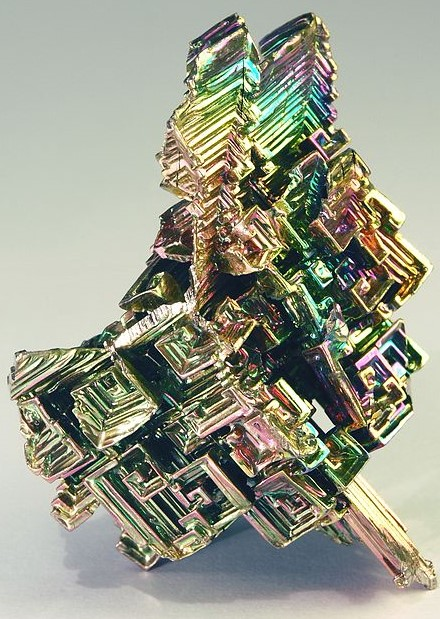
\includegraphics[height=3.5cm]{bismuth.jpg}
            \caption{Bismuth. Image credit: \copyright{}Micha L. Rieser {\scriptsize \url{https://commons.wikimedia.org/wiki/File:Bismuth-crystal.jpg}.}}
        \end{subfigure}
        \begin{subfigure}[t]{0.4\textwidth}
            \centering
            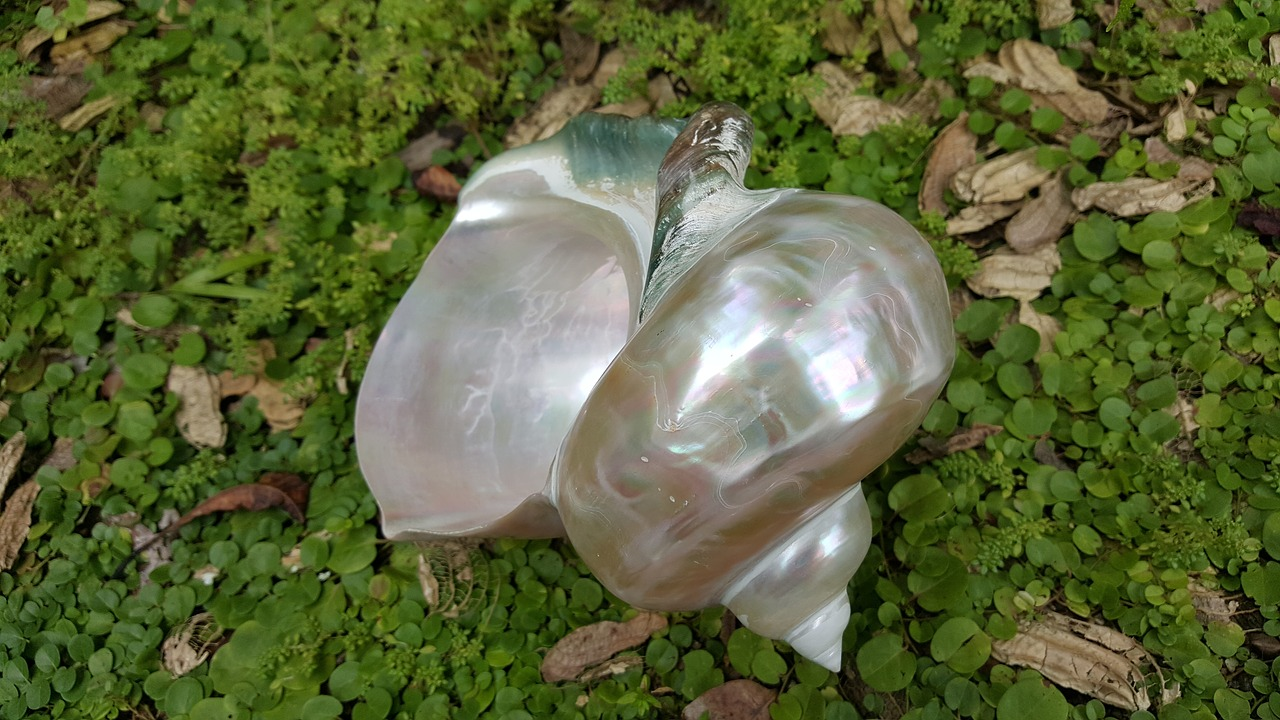
\includegraphics[height=3.5cm]{shell.jpg}
            \caption{Shell. Image credit: {\scriptsize \url{https://pixabay.com/photos/pearl-fire-oud-shells-nautilus-sea-1602541/}.}}
        \end{subfigure}
        \begin{subfigure}[t]{0.3\textwidth}
            \centering
            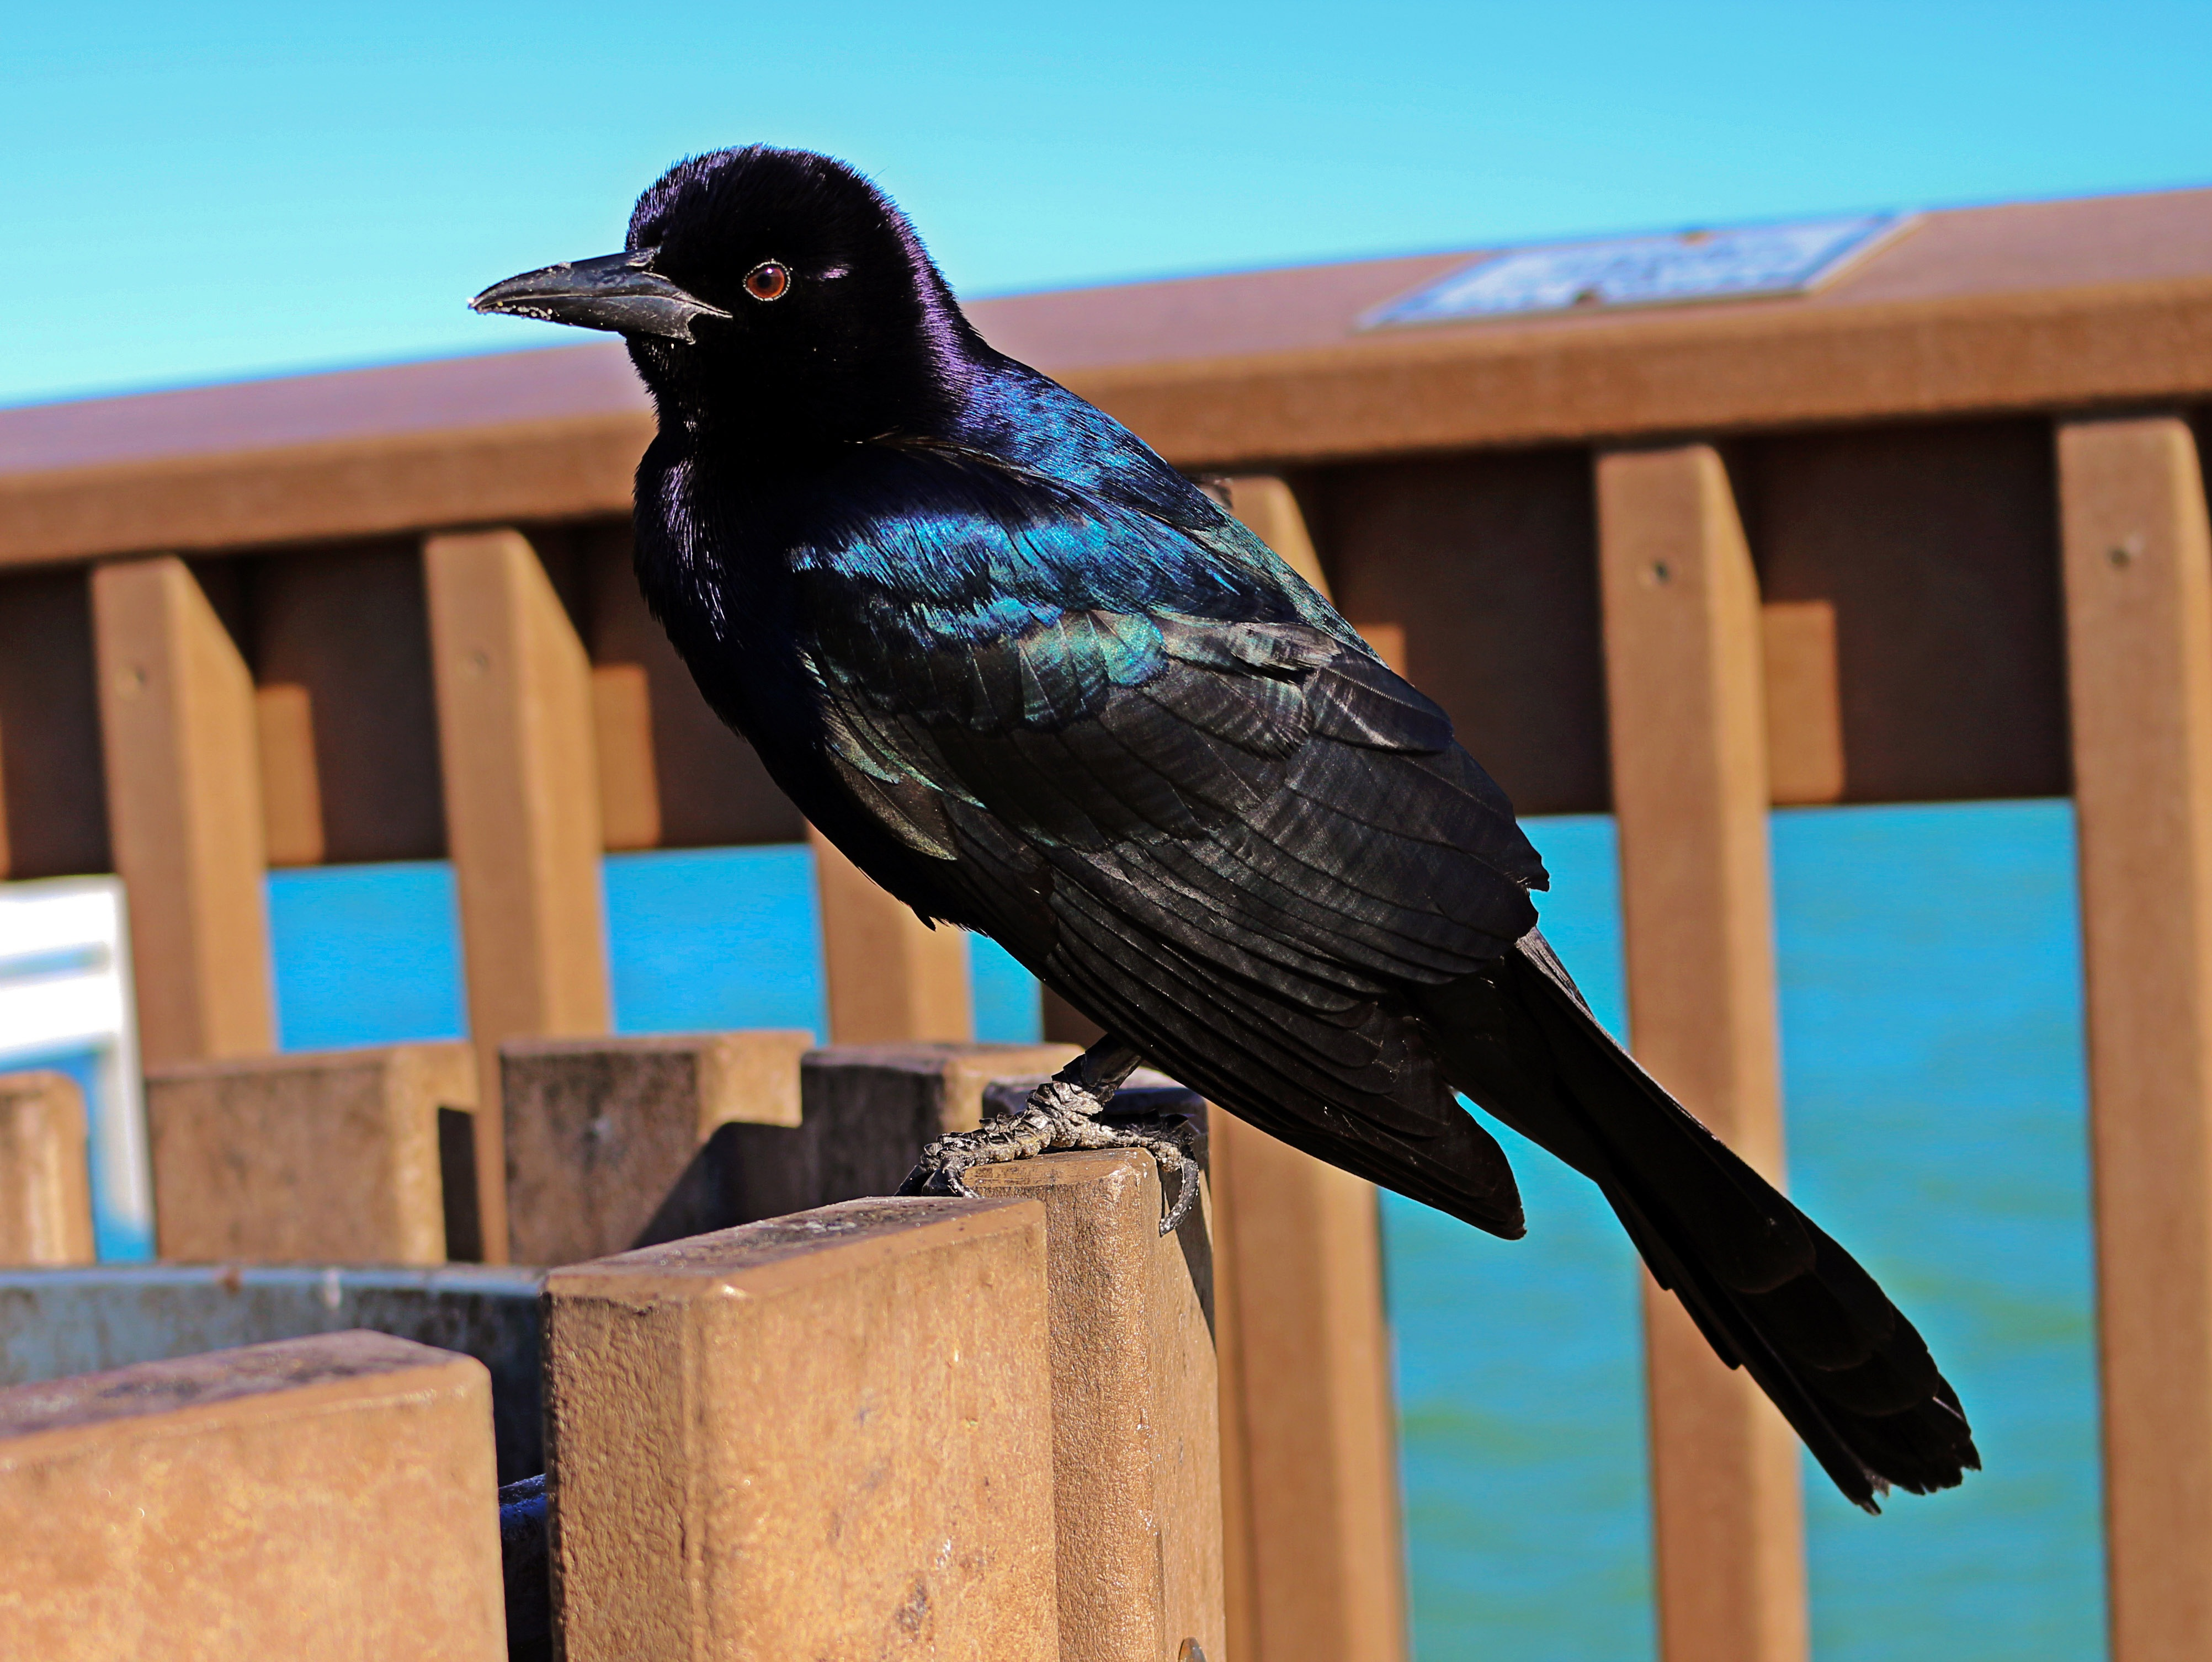
\includegraphics[height=3.5cm]{bird.jpg}
            \caption{Bird. Image credit: {\scriptsize \url{https://pxhere.com/en/photo/653981}.}}
        \end{subfigure}
        \caption{Some natural examples of thin films causing iridescence.}
    \end{figure}

    \subsection{Multiple Reflections}
    Up to now we have assumed that all secondary reflections are sufficiently weak that they can be ignored.
    This isn't the case for a non-transparent material and is only an approximation for a transparent material.
    
    Consider an air-film-glass setup.
    The first reflection off of the air-film boundary has reflection coefficient \(r_1 = r_{af}\).
    The second reflection is off of the film-glass boundary and has reflection coefficient 
    \[r_2 = t_{af}e^{i\beta}r_{fg}e^{i\beta}t_{fa}.\]
    The factor of \(t_{af}\) accounts for the fact that this ray is first transmitted at the air-film boundary.
    It then travels through the medium picking up a phase factor of \(e^{i\beta}\) (\(\beta = 2\pi n_fd\cos\vartheta_t/\lambda\)).
    It is then reflected at the film-glass boundary picking up a factor of \(r_{fg}\), travels back through the film picking up another \(e^{i\beta}\) and finally is transmitted at the film-air boundary picking up a factor of \(t_{fa}\).
    The third reflection follows almost the same path but instead of being transmitted at the film-air boundary it is reflected \((r_{fa})\), travels back through the film \((e^{i\beta})\), is reflected at the film-glass boundary \((r_{fg})\), travels back through the film, \((e^{i\beta})\), and is finally transmitted at the film-air boundary \((t_{fa})\).
    So the third ray to leave the film into the air has reflection coefficient
    \begin{align*}
        r_3 &= t_{af}e^{i\beta}r_{fg}e^{i\beta}(r_{fa}e^{i\beta}r_{fg}e^{i\beta})t_{fa}\\
        &= r_2(r_{fa}e^{2i\beta}r_{fg}).
    \end{align*}
    By the same logic we can write the reflection coefficient for the fourth reflected ray as
    \[r_{4} = r_3x = r_2x^2, \qquad\text{where}\qquad x = f_{fa}e^{2i\beta}r_{fg}.\]
    Continuing \textit{ad infinitum} we see that the total reflection coefficient is
    \[r_{afg} = r_1 + r_2(1 + x + x^2 + \dotsb) = r_1 + \frac{r_2}{1 - x}.\]
    In the last step we have identified the geometric series which converges if and only if \(\abs{x} < 1\).
    It can be shown then that
    \[f_{afg} = \frac{r_{af} + r_{fg}e^{2i\beta}}{1 + r_{af}}r_{fg}e^{2i\beta}.\]
    
    Suppose we have an unsupported thin film, that is the film has the same medium on either side (as opposed to being layered onto glass).
    For simplicity we will also assume that this medium is air.
    Then
    \[f_{afa} = \frac{r_{af} + r_{fa}e^{2i\beta}}{1 + r_{af}r_{fa}e^{2i\beta}} = \frac{r_{af} - r_{af}e^{2i\beta}}{1 - r_{af}r_{af}e^{2i\beta}} = \frac{r[1 - e^{2i\beta}]}{1 - r^2e^{2-\beta}}\]
    where we right \(r = r_{af}\) for brevity.
    The reflectivity of the film is then
    \begin{align*}
        R &= \abs{r_{afa}}^2\\
        &= \frac{r[1 - e^{2i\beta}]}{1 - r^2e^{2i\beta}}\frac{r[1 - e^{-2i\beta}]}{1 - r^2e^{-2i\beta}}\\
        &= \frac{2r^2[1 - \cos(2\beta)]}{1 - 2r^2\cos(2\beta) + r^4}.
    \end{align*}
    We assumed here that \(r\in\reals\) which means that \(n\in\reals\) which means that we are considering only transparent, non-absorbing, materials.
    We then have that the transmissivity is
    \[T = 1 - R = \frac{(1 - r)^2}{1 - 2r^2\cos(2\beta) + r^4}.\]
    This is minimised when \(\cos(2\beta) = -1\) so \(4\pi n_fd\cos\vartheta_t/\lambda = (2m - 1)\pi\) for \(m\in\integers\).
    We find that
    \[\min\{T\} = \frac{(1 - r^2)^2}{(1 + r^2)^2}\]
    and
    \[\max\{R\} = 1 - \min\{T\} = \frac{4r^2}{(1 + r^2)^2}.\]
    We can introduce the \define{Finesse coefficient}, \(F\), here defined as
    \[F = \left( \frac{2r}{1 - r^2} \right)^2\]
    which allows us to write
    \[R = \frac{F\sin^2\beta}{1 + F\sin^2\beta}, \qquad\text{and}\qquad T = \frac{1}{1 + F\sin^2\beta}.\]
    For small \(r\) we have an approximately \(\sin^2\) fringe pattern, just as we observed for two beam interference.
    For larger values of \(r\) however we have strong multiple reflections and a more complex fringe pattern.
    As \(r \to 1\) we have \(T \to 0\) and \(R \to 1\) unless \(\beta = m\pi\) for some \(m\in\integers\) in which case we have narrow bands which appear bright viewing with the source on the other side of the film or as dark viewing on the same side as the source.
    \(R\) and \(T\) plotted for various values of \(r\), \(F\), and \(\beta\) can be seen in figure~\ref{fig:reflectivity and transmissivity}.
    
    \begin{figure}[htbp!]
        \centering
        \begin{subfigure}{0.9\textwidth}
            \centering
            \tikzsetnextfilename{thin-film-reflectivity}
            \begin{tikzpicture}
                \tikzset{myplot/.style={ultra thick}}
                \begin{axis}[
                    domain=0:4*pi,
                    xlabel=\(\beta\),
                    ylabel=\(R\),
                    xtick={
                        0, pi, 2*pi, 3*pi, 4*pi
                    },
                    xticklabels={
                        0, \(\pi\), \(2\pi\), \(3\pi\), \(4\pi\)
                    },
                    samples=300
                    ]
                    % Plots
                    \addplot[
                    myplot,
                    red
                    ] {1 - 1 / (1 + 0.22 * sin(deg(x))^2)};  % r^2 = 0.05, F= 0.22
                    \addplot[
                    myplot,
                    red!50!blue,
                    dashed
                    ] {1 - 1 / (1 + 1.25 * sin(deg(x))^2)};  % r^2 = 0.2, F = 1.25
                    \addplot[
                    myplot,
                    blue,
                    dotted
                    ] {1 - 1 / (1 + 80 * sin(deg(x))^2)};  % r^2 = 0.8, F = 80
                    
                    % Guide lines
                    \draw[dashed, thick, gray] (0, 1) -- (4*pi, 1);
                    \draw[dashed, thick, gray] (pi, 1) -- (4*pi, 1);
                    \draw[dashed, thick, gray] (0, 0) -- (0, 1);
                    \draw[dashed, thick, gray] (pi, 0) -- (pi, 1);
                    \draw[dashed, thick, gray] (2*pi, 0) -- (2*pi, 1);
                    \draw[dashed, thick, gray] (3*pi, 0) -- (3*pi, 1);
                    \draw[dashed, thick, gray] (4*pi, 0) -- (4*pi, 1);
                    
                    % Legend
                    \addlegendentry{\tiny\(r^2 = 0.05\), \(F = 0.22\)}
                    \addlegendentry{\tiny\(r^2 = 0.2\), \(F = 1.25\)}
                    \addlegendentry{\tiny\(r^2 = 0.8\), \(F = 80\)}
                \end{axis}
            \end{tikzpicture}
            \caption{The reflectivity, \(R\).}
        \end{subfigure}
        \begin{subfigure}{0.9\textwidth}
            \centering
            \tikzsetnextfilename{thin-film-transmissivity}
            \begin{tikzpicture}
                \tikzset{myplot/.style={ultra thick}}
                \begin{axis}[
                    domain=0:4*pi,
                    xlabel=\(\beta\),
                    ylabel=\(T\),
                    xtick={
                        0, pi, 2*pi, 3*pi, 4*pi
                    },
                    xticklabels={
                        0, \(\pi\), \(2\pi\), \(3\pi\), \(4\pi\)
                    },
                    samples=300,
                    legend pos=south east
                    ]
                    % Plots
                    \addplot[
                    myplot,
                    red
                    ] {1 / (1 + 0.22 * sin(deg(x))^2)};  % r^2 = 0.05, F= 0.22
                    \addplot[
                    myplot,
                    red!50!blue,
                    dashed
                    ] {1 / (1 + 1.25 * sin(deg(x))^2)};  % r^2 = 0.2, F = 1.25
                    \addplot[
                    myplot,
                    blue,
                    dotted
                    ] {1 / (1 + 80 * sin(deg(x))^2)};  % r^2 = 0.8, F = 80
                    
                    % Guide lines
                    \draw[dashed, thick, gray] (0, 1) -- (4*pi, 1);
                    \draw[dashed, thick, gray] (pi, 1) -- (4*pi, 1);
                    \draw[dashed, thick, gray] (0, 0) -- (0, 1);
                    \draw[dashed, thick, gray] (pi, 0) -- (pi, 1);
                    \draw[dashed, thick, gray] (2*pi, 0) -- (2*pi, 1);
                    \draw[dashed, thick, gray] (3*pi, 0) -- (3*pi, 1);
                    \draw[dashed, thick, gray] (4*pi, 0) -- (4*pi, 1);
                    
                    % Legend
                    \addlegendentry{\tiny\(r^2 = 0.05\), \(F = 0.22\)}
                    \addlegendentry{\tiny\(r^2 = 0.2\), \(F = 1.25\)}
                    \addlegendentry{\tiny\(r^2 = 0.8\), \(F = 80\)}
                \end{axis}
            \end{tikzpicture}
            \caption{The transmissivity, \(T\).}
        \end{subfigure}
        \caption{The reflectivity and transmissivity, \(R\) and \(T\), for an unsupported thin film in air.}
        \label{fig:reflectivity and transmissivity}
    \end{figure}
    
    For high values of \(r\) or \(F\) the transmissivity is very selective for specific values of \(\beta\), and hence for specific wavelengths.
    This is exploited in \define{Fabry-Perot} systems which are comprised of two parallel highly reflective surfaces, usually dielectric mirrors made with multiple layers of thin films.
    The two mirrors are separated by a distance \(d\) and filled with a medium of refractive index \(n\).
    If the cavity is then illuminated by a collimated beam (that is light where all rays are parallel) of amplitude \(E_0\) which enters at angle \(\vartheta_0\) to the normals of the mirrors.
    If we choose \(\vartheta_0 = 0\) then we will get transmission of wavelengths close to
    \[\lambda_m = \frac{2nd}{m}\]
    where \(m\in\integers\).
    This corresponds to a half-integer number of wavelengths fitting in the cavity.
    The result is that only light within a very narrow range around these key values of \(\lambda_m\) can pass out of the cavity so it acts as a very narrow bandpass filter.